\documentclass[tikz,border=8pt]{standalone}
\usepackage{tikz}
\usetikzlibrary{positioning, arrows.meta}

\begin{document}
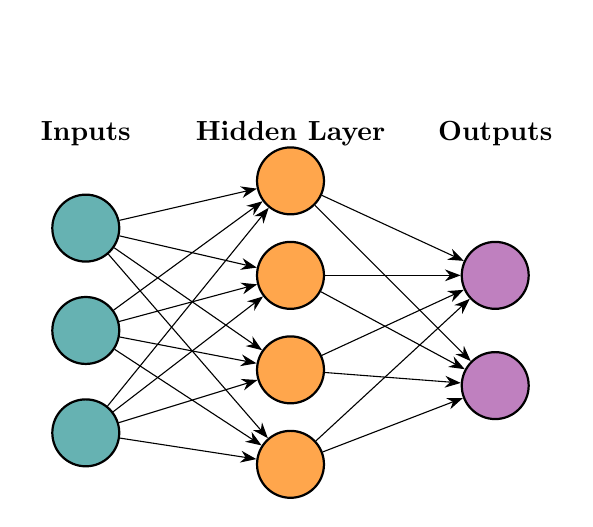
\begin{tikzpicture}[
    every node/.style = {circle, draw=black, thick, minimum size=0.85cm},
    input/.style  = {fill=teal!60},
    hidden/.style = {fill=orange!70},
    output/.style = {fill=violet!50},
    label/.style  = {draw=none, fill=none, font=\bfseries},
    >={Stealth[length=2mm]}
]

% input layer
\node[input] (i1) at (0, 0)   {};
\node[input] (i2) at (0, -1.3) {};
\node[input] (i3) at (0, -2.6) {};

% hidden layer
\node[hidden] (h1) at (2.6, 0.6)   {};
\node[hidden] (h2) at (2.6, -0.6)  {};
\node[hidden] (h3) at (2.6, -1.8)  {};
\node[hidden] (h4) at (2.6, -3.0)  {};

% output layer
\node[output] (o1) at (5.2, -0.6)  {};
\node[output] (o2) at (5.2, -2.0)  {};

% layer labels, all at the same height
\node[label] at (0,   1.2) {Inputs};
\node[label] at (2.6, 1.2) {Hidden Layer};
\node[label] at (5.2, 1.2) {Outputs};

% connections: input -> hidden
\foreach \i in {1,2,3}
    \foreach \h in {1,2,3,4}
        \draw[->] (i\i) -- (h\h);

% connections: hidden -> output
\foreach \h in {1,2,3,4}
    \foreach \o in {1,2}
        \draw[->] (h\h) -- (o\o);

\end{tikzpicture}
\end{document}
